\chapter{When Hard Work Misses the Basics}

This chapter follows a short School of Hard Knocks interview segment, curated for this book by LazyingArt LLC through Video2Book. The question is simple: what did football teach that later mattered in business? The answer does not begin with a formula, a balance sheet, or a heroic success story. It begins with a mistake: the speaker worked hard, had strong coaches, and still did not get everything he could have gotten from the game because he kept trying to do things his own way.

\section{The Transfer Question}

The interview opens with a question about transfer. The speaker is asked what lesson from football helped him become the business owner and leader he is today. That framing matters. We are not merely collecting a sports anecdote; we are asking how a habit learned in one domain becomes useful in another.

A weak answer would say only that sports build character. The speaker begins near that answer, but he does not stay there. The useful lesson is more precise. Football gave him a way to see the difference between exertion and disciplined learning.

\section{The Expected Lessons}

The first answer is the familiar one. In football, one learns to work with a team and to deal with adversity. Those are real lessons, and the speaker does not dismiss them. But he treats them as the common answer, the kind of answer anyone could give about sports.

That move sets up the deeper point. Teamwork and adversity are broad categories. They describe the atmosphere of competitive sport. The speaker wants to identify the particular failure that taught him something sharper.

\begin{remark}
For the purposes of the entrepreneurship chapter, the broad lessons should remain in the text, but they should not be inflated. They are the baseline. The distinctive lesson comes next.
\end{remark}

\section{The Lesson Came From Mistakes}

The speaker then pivots: the best lesson came from his mistakes in sports. This is the first important turn in the lecture's rhythm. The lesson is not presented as a trophy from football, but as a later understanding of something he handled poorly.

That distinction is central for business. A mistake becomes useful only when it can be inspected without decoration. Here the mistake is not laziness, lack of effort, or lack of opportunity. It is a mismatch between effort and receptivity.

\section{Quarterback, College, and Coaches}

The speaker identifies himself as a quarterback, specifically a scrappy dual-threat quarterback. The role matters because quarterbacking is a decision-making position. A quarterback must execute, adapt, and still remain inside the structure of the play.

The setting is Long Beach City College, a junior college just outside Los Angeles. He names two coaches, Brad Peabody and Ryan Flynn, and describes them as exceptional. The names should stay in the chapter because they keep the account from becoming generic. The speaker is not saying, in the abstract, that people should listen to mentors. He is describing a concrete period in which capable coaches were trying to teach him.

\begin{definition}
In this chapter, a \emph{basic} means a fundamental practice or principle that is already known to competent teachers but must still be accepted, repeated, and applied by the learner. A basic is not beneath the work. It is the structure that lets hard work compound.
\end{definition}

\section{Hard Work Without Basics}

The conflict arrives after the coaches are established. The problem was not that the speaker lacked guidance. The problem was that he was obsessed with doing everything his own way. He does not quite say that he knew more than his coaches; the point is subtler and more common. They would teach him, and he would keep trying to make the work conform to his own preferred method.

The result was a failure to stick to the basics. He worked very hard, but he did not fully use his brain in the way he could have. That line should be read carefully. It is not an argument against effort. It is an argument against effort that refuses correction.

\subsection{Question \& Answer}

\paragraph{Question.}
If he worked very, very, very hard, why was that not enough?

\paragraph{Answer.}
Because effort does not automatically become learning. In the speaker's account, the missing ingredient was disciplined receptivity: the willingness to take coaching seriously, stay with the basics, and let judgment govern the work. The mistake was not low intensity. The mistake was self-directed intensity without enough obedience to fundamentals.

\begin{figure}
\centering
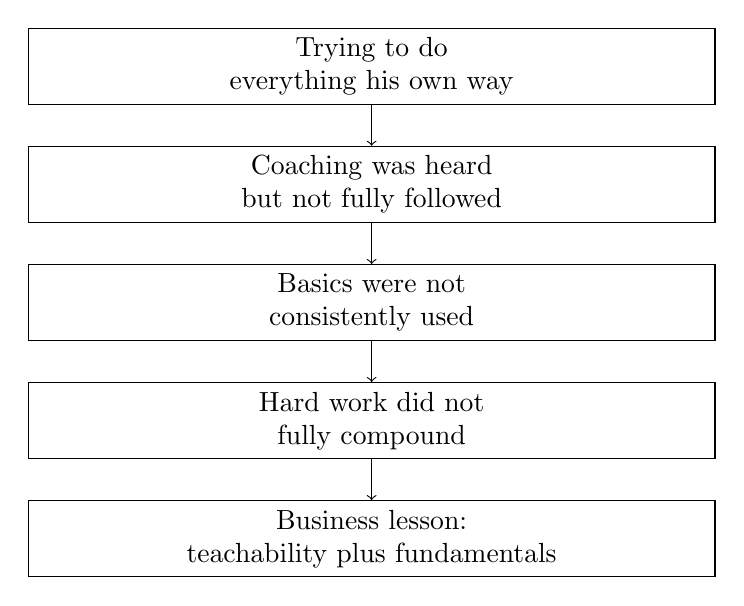
\begin{tikzpicture}[x=1cm,y=1cm]
\node[draw, align=center, text width=0.70\linewidth] (a) at (0,0) {Trying to do\\everything his own way};
\node[draw, align=center, text width=0.70\linewidth] (b) at (0,-1.5) {Coaching was heard\\but not fully followed};
\node[draw, align=center, text width=0.70\linewidth] (c) at (0,-3.0) {Basics were not\\consistently used};
\node[draw, align=center, text width=0.70\linewidth] (d) at (0,-4.5) {Hard work did not\\fully compound};
\node[draw, align=center, text width=0.70\linewidth] (e) at (0,-6.0) {Business lesson:\\teachability plus fundamentals};
\draw[->] (a) -- (b);
\draw[->] (b) -- (c);
\draw[->] (c) -- (d);
\draw[->] (d) -- (e);
\end{tikzpicture}
\caption{A transcript-backed reconstruction of the lesson: the speaker's mistake was not lack of work, but work separated from coachability and basics.}
\end{figure}

The diagram is not a board figure from the video. It is a compact reconstruction of the spoken mechanism. Its job is to preserve the causal order of the answer: own way, ignored coaching, missed basics, underused hard work, business lesson.

\section{From Football Mistake to Business Judgment}

The business implication should be stated cautiously, because this excerpt stops at the diagnosis. Still, the mechanism is clear enough. A leader can be energetic and still be untrained in the places that matter. Drive is useful, but drive becomes dangerous when it treats correction as interference.

The football story therefore contributes to the broader entrepreneurship book under judgment, operations, and resilience. It is about judgment because the speaker had to learn that his own instincts were not always the highest authority. It is about operations because basics are the repeatable parts of performance. It is about resilience because the valuable lesson came from admitting that past effort had been incomplete.

The lesson is not that a business owner should blindly follow every adviser. The transcript does not support that broad claim. The narrower claim is stronger: when capable teachers are present, and when the basics are known, refusing to submit one's work to those basics can waste even sincere effort.

\section{Summary}

The interview begins with the expected bridge from football to business: teamwork and adversity. It then turns toward the real lesson, which came from mistakes. As a quarterback at Long Beach City College, working with Brad Peabody and Ryan Flynn, the speaker had strong coaching available, but he kept trying to do things his own way.

The chapter's durable point is that hard work is not self-justifying. In business, as in sport, effort has to be joined to basics, instruction, and judgment. Otherwise a person can work intensely and still leave much of his ability unused.